\documentclass{article}
\usepackage{geometry}
\geometry{left=2cm,right=2cm,top=2cm,bottom=2cm}

\usepackage{graphicx}
\graphicspath{{pics/}}

\setlength{\arrayrulewidth}{0.3mm}
\setlength{\tabcolsep}{18pt}
\renewcommand{\arraystretch}{1.3}

\usepackage{caption}
\usepackage{subcaption}
\begin{document}

\title{Assignment 1}
\author{Weiqi Luo \ 03697059}

\maketitle
\newpage

\section*{Exercise 1}

\subsection*{Exercise 1.a - 1.b}
\subsubsection*{k=2}
(1) Optimal value of p1, p2 :  \\
\begin{center}
	\begin{tabular}{ l | c }
		\hline
		p1 & p2 \\ \hline		
		5 & 3 \\ \hline
	\end{tabular}
\end{center}
(2) Learned parameter values : \\
\begin{center}
	\begin{tabular}{ l | c | r  }
		\hline
		par\{1,1\}& par\{1,2\} & par\{1,3\} \\
		\hline		
	   2.2063e-03 & -2.6949e-03 & -5.9515e-04 \\ \hline
	   9.2173e-01 & -1.3581e-03 & -1.7107e-04 \\ \hline
	   6.5735e-03 & -1.1538e-02 & 9.9971e-01 \\ \hline
	   -1.6266e-03 & 4.7304e-01 & 8.3936e-04 \\ \hline
	   -9.9158e-04 & 2.4454e-04 & 1.2687e-04 \\ \hline
	   2.4849e-03 & -8.2673e-03 & 1.7827e-03 \\ \hline
	   2.3136e-03 & 7.4693e-05 & -1.4105e-04 \\ \hline
	   -1.1665e-05 & 4.3810e-05 & -4.5223e-06 \\ \hline
	   -1.3006e-02 & 1.6437e-02 & -6.2224e-04 \\ \hline
	   1.2268e-04 & -9.7700e-04 & -1.3221e-05 \\ \hline
	   1.2836e-05 & -5.2889e-06 &  \\ \hline
	   -4.4566e-03 & 4.2985e-03 &  \\ \hline
	   -4.3099e-05 & -4.4187e-06 &  \\ \hline
	   1.6696e-06 & -2.6911e-07 &  \\ \hline
	   2.5977e-03 & -3.8127e-03 &  \\ \hline
	   -4.0239e-07 & 2.1016e-06 &  \\ \hline
	\end{tabular}
\end{center}
\newpage
\subsubsection*{k=5}
(1) Optimal value of p1, p2 :  \\
\begin{center}
	\begin{tabular}{ l | c }
		\hline
		p1 & p2 \\ \hline		
		4 & 1 \\ \hline
	\end{tabular}
\end{center}
(2) Learned parameter values : \\
\begin{center}
	\begin{tabular}{ l | c | r  }
		\hline
		par\{1,1\}& par\{1,2\} & par\{1,3\} \\
		\hline		
		2.5044e-03 & -4.3238e-03 & 8.0784e-04 \\ \hline
		9.1976e-01 & -1.0015e-03 & -3.1902e-04 \\ \hline
		-2.8554e-03 & 1.4480e-03 & 9.9870e-01 \\ \hline
		-7.4385e-04 & 4.6798e-01 & 3.2142e-04 \\ \hline
		-1.0342e-03 & 5.6850e-04 &  \\ \hline
		1.3743e-03 & -2.5277e-03 &  \\ \hline
		2.4869e-03 & -1.0251e-03 &  \\ \hline
		1.3601e-04 & 1.9246e-05 &  \\ \hline
		-2.6908e-04 & -1.6742e-03 &  \\ \hline
		6.6926e-05 & -6.7254e-04 &  \\ \hline
		1.3061e-05 & -7.8462e-06 &  \\ \hline
		-4.2816e-03 & 3.4766e-03 &  \\ \hline
		-4.5174e-05 & 8.7155e-06 &  \\ \hline
	\end{tabular}
\end{center}

\newpage
\subsection*{Exercise 1.c}
\begin{figure}[ht]
	\begin{subfigure}{.5\textwidth}
		\centering
		% include first image
		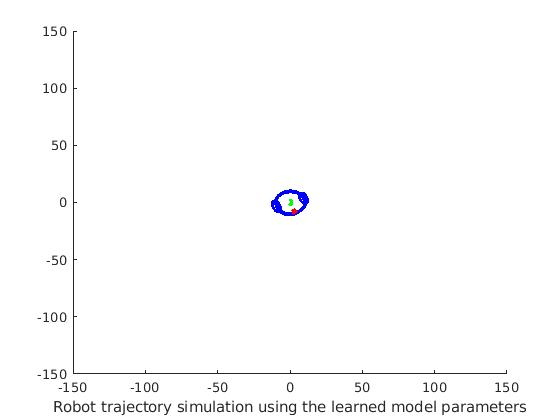
\includegraphics[width=1.\linewidth]{1.jpg}  
		\caption{Simulation (v, w) = (0, 0.05)}
	\end{subfigure}
	\begin{subfigure}{.5\textwidth}
		\centering
		% include second image
		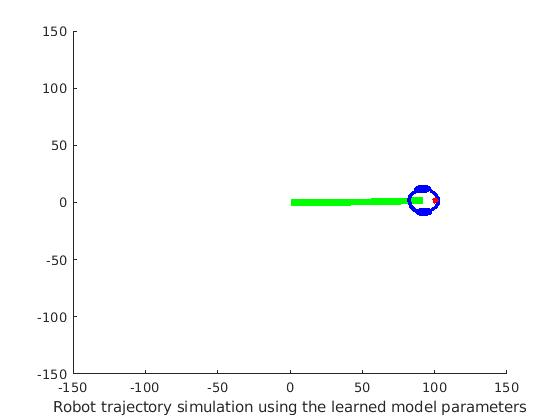
\includegraphics[width=1.\linewidth]{2.jpg}  
		\caption{Simulation (v, w) = (1, 0)}
	\end{subfigure}
	\begin{subfigure}{.5\textwidth}
		\centering
		% include first image
		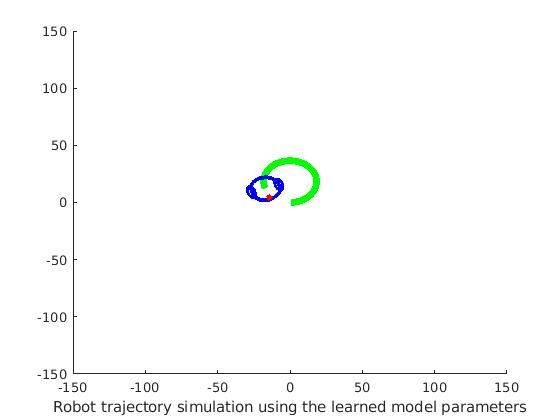
\includegraphics[width=1.\linewidth]{3.jpg}  
		\caption{Simulation (v, w) = (1, 0.05)}
	\end{subfigure}
	\begin{subfigure}{.5\textwidth}
		\centering
		% include second image
		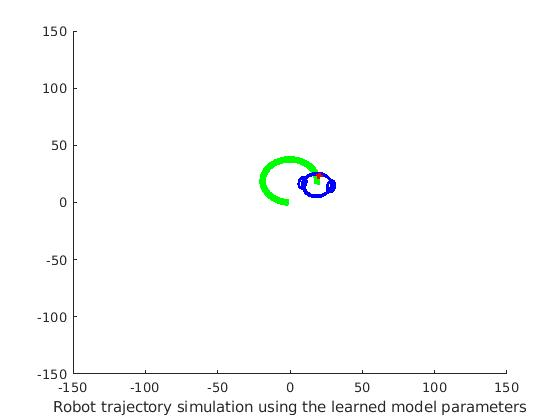
\includegraphics[width=1.\linewidth]{4.jpg}  
		\caption{Simulation (v, w) = (-1, -0.05)}
	\end{subfigure}
\end{figure}
\newpage
\section*{Exercise 2}
(1) The optimized number of principal components and respective classification error:
\begin{center}
	\begin{tabular}{ l | c }
		\hline
		$d_{opt}$ & $err_{min}$ \\ \hline		
		$48$ & $3.620\%$ \\ \hline
	\end{tabular}
\end{center}
(2) confusion matrix:
\begin{figure}[ht]
	\centering
	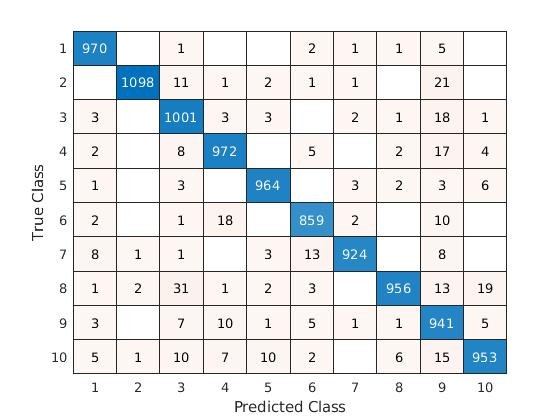
\includegraphics[width=0.7\linewidth]{confusionMat.jpg}  
\end{figure}
\\[8pt]
\begin{figure}[ht]
	\centering
	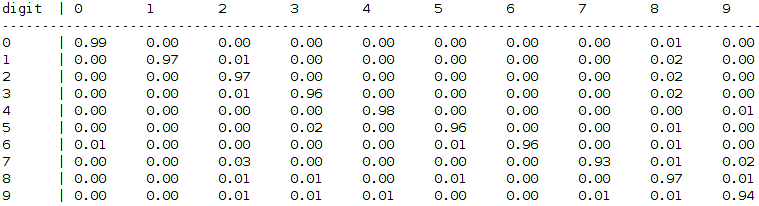
\includegraphics[width=1\linewidth]{helper.png}  
\end{figure}
\newpage
(3) plot of classification error:
\begin{figure}[ht]
	\centering
	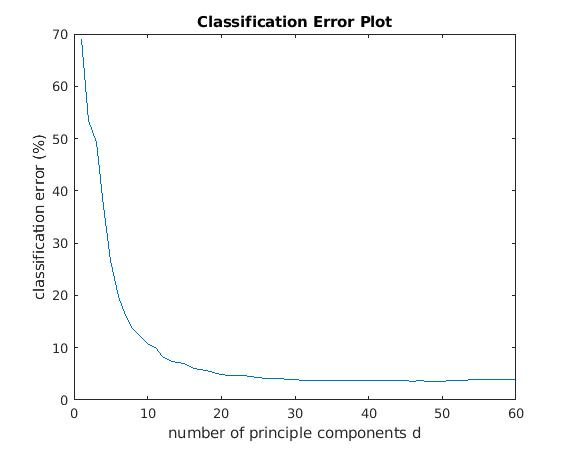
\includegraphics[width=0.8\linewidth]{error.jpg}  
\end{figure}

\newpage
\section*{Exercise 3}
\begin{figure}[ht]
	\begin{subfigure}{.5\textwidth}
		\centering
		% include first image
		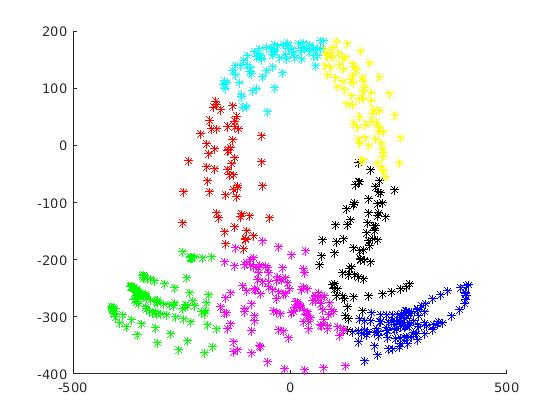
\includegraphics[width=1.\linewidth]{kmean1.jpg}  
		\caption{gesture l clustering using kmeans}
	\end{subfigure}
	\begin{subfigure}{.5\textwidth}
		\centering
		% include second image
		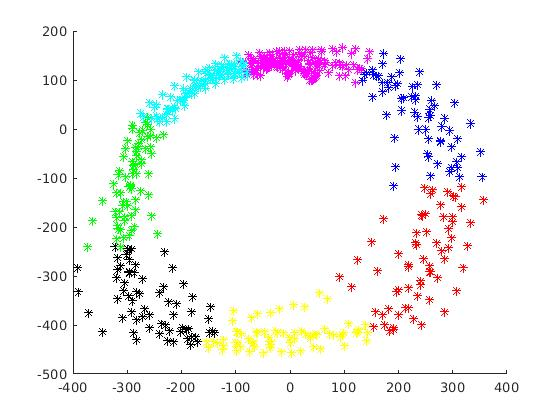
\includegraphics[width=1.\linewidth]{kmean2.jpg}  
		\caption{gesture o clustering using kmeans}
	\end{subfigure}
	\begin{subfigure}{.5\textwidth}
		\centering
		% include first image
		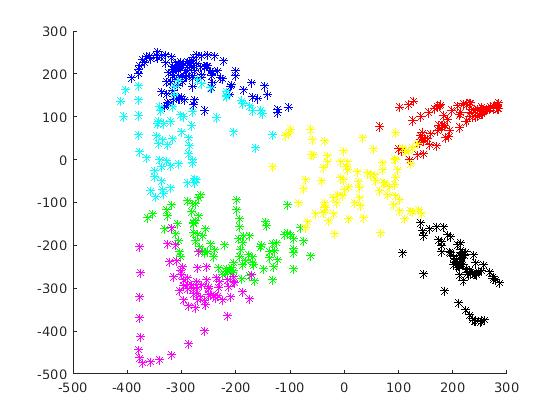
\includegraphics[width=1.\linewidth]{kmean3.jpg}  
		\caption{gesture x clustering using kmeans}
	\end{subfigure}
\end{figure}
\end{document}